
In all of our experiments we use the same training settings used in~\cite{Kingma2014}; that is,  
we use Adagrad for optimization with minibatches of 100  with a learning rate of 0.01
and a weight decay corresponding to a prior of $\mathcal{N}(0,1)$.
We initialize weights in our network using the heuristic of ~\cite{glorot2010understanding}.
However for the pose recognition modules in the ST-VAE model, we have found it useful to
specifically initialize biases so that poses are initially close to the identity transformation (see~\cite{jaderberg2015spatial}).

For all three models (VAE, ST-VAE, CST-VAE),
we experiment with between 10 and 50  dimensions for the latent variables $z$.
We parameterize content encoders and decoders
by using a two layer fully connected MLP with 256 dimensional
hidden layers and ReLU nonlinearities.
For pose decoders and encoders we also use two layer fully connected MLPs, but 
using 32 dimensional hidden layers and Tanh nonlinearities.\footnote{
In practice, we have found this choice of Tanh vs. ReLU makes a significant difference in practice}
Finally for spatial transformer modules, we always resample onto a grid that is the same size as the original
image.


\Jon{For binary images, it is common to have a sigmoid at the end of the VAE decoder.
However we have found that it is often more numerically stable in these situations to first apple the spatial transformation, then
to apply the sigmoid after the transformation.
}

\subsection{Evaluating the Spatially transformed Variational Autoencoder alone}

We first evaluate our ST-VAE model alone on the MNIST dataset~\citep{lecun1998gradient}
and a derived dataset, \emph{TranslatedMNIST}, in which we randomly translated each  $28\times 28$ MNIST example
within a $36\times 36$ black image.  In both cases, we binarize the images by thresholding at value 128.



Ordinary and Translated MNIST comparing
\begin{itemize}
\item ordinary vae
\item stvae model
\end{itemize}


\begin{itemize}
\item show pretty images
\item show that we often converge in first few iterations in pose and start to learn style after that
\end{itemize}



\Jon{Accuracy of classification of latent layer?}



\begin{figure}[t]
\begin{center}
\subfigure[]{
\raisebox{3mm}{
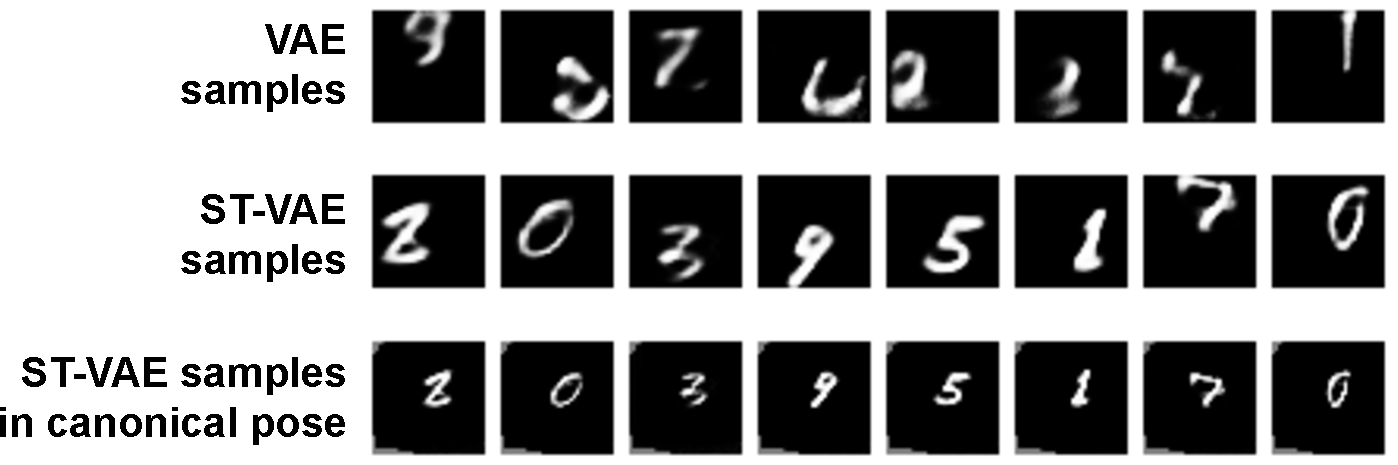
\includegraphics[width=0.45\linewidth]{figs/vae_stvae_samples.pdf}
\label{fig:vae_stvae_samples}
}
}
\qquad
\subfigure[]{
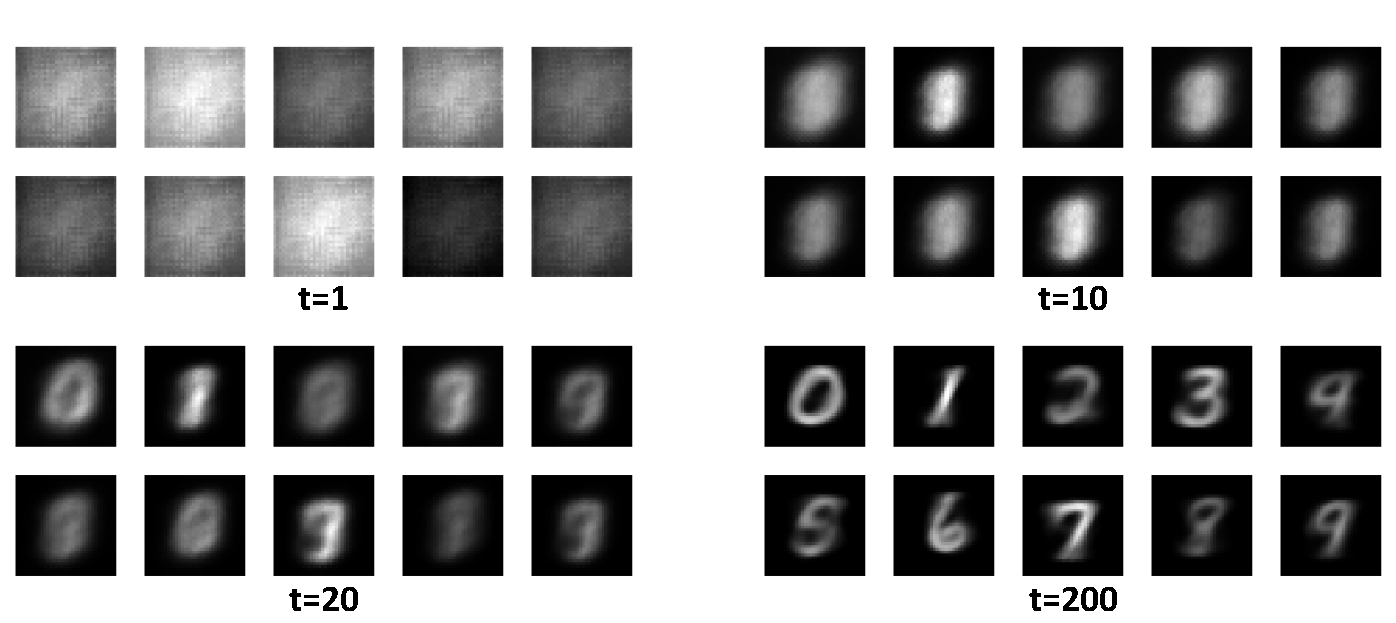
\includegraphics[width=0.45\linewidth]{figs/stvae_averageddigits.pdf}
\label{fig:stvae_averageddigits}
}
\end{center}
 \caption{hello}
\end{figure}

\begin{figure}[t]
\begin{center}
\subfigure[]{
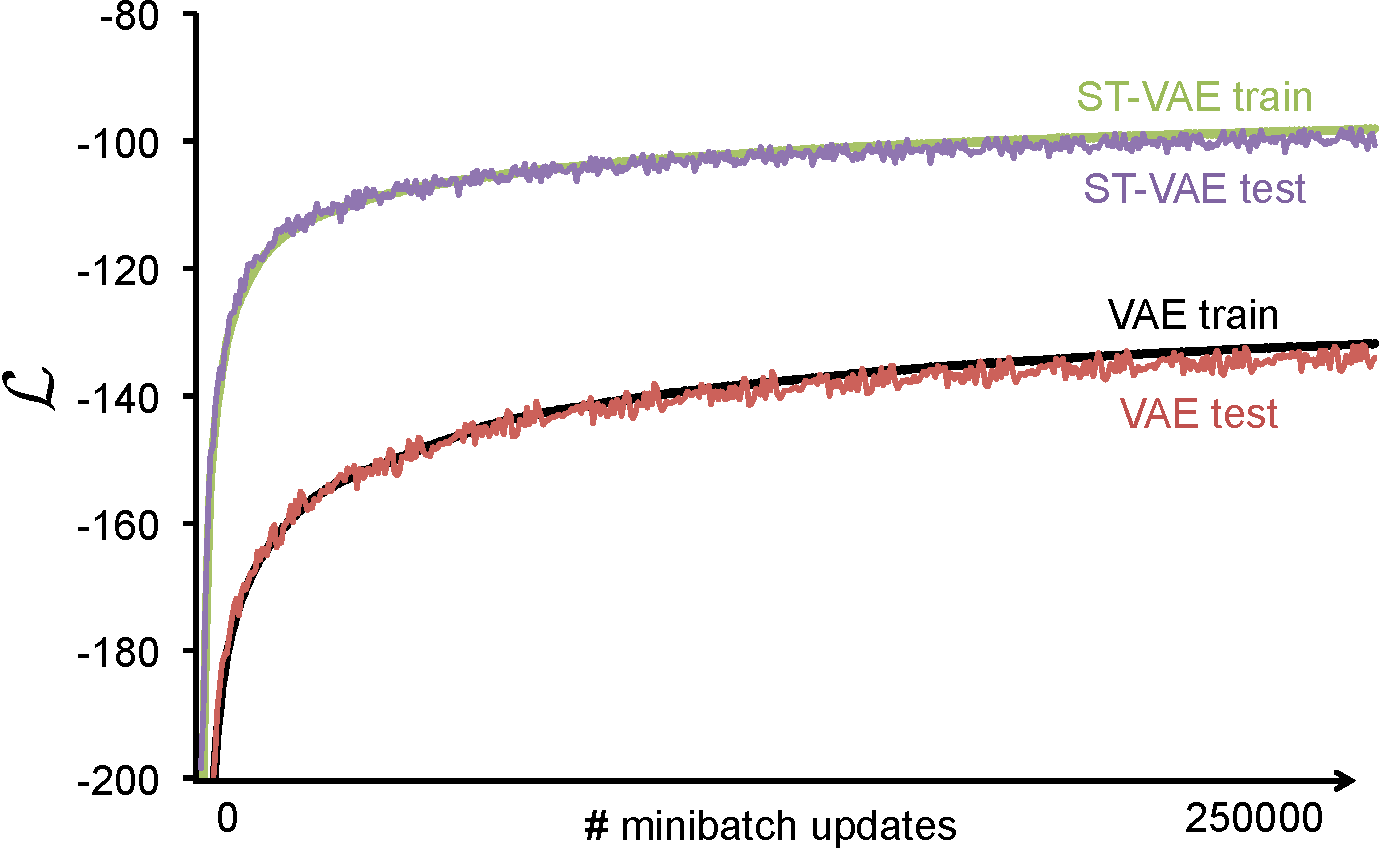
\includegraphics[width=0.30\linewidth]{figs/vae_stvae_learning_curves.pdf}
\label{fig:vae_stvae_learning_curves}
}
\subfigure[]{
\raisebox{12mm}{
\footnotesize
\begin{tabular}{lcc} 
\hline 
%\multicolumn{1}{r|}{Proposals} & \multicolumn{2}{c}{GT} & \multicolumn{2}{c}{multibox} \\
%\multicolumn{1}{r|}{Descriptions} & GEN & GT & GEN & GT \\
 & Train Accuracy & Test Accuracy \\
\hline 
\multicolumn{3}{l}{On translated (36x36) MNIST} \\
\hline
VAE + supervised & 0.771 & 0.146 \\
ST-VAE + supervised & 0.972 & 0.964  \\
directly supervised & 0.884 & 0.783 \\
Directly supervised with STN & 0.993 & 0.969  \\
\hline 
\multicolumn{3}{l}{On original (28x28) MNIST} \\
\hline 
Directly supervised & 0.999 & 0.96   \\
\hline
\end{tabular}%
}
}
\end{center}

 \caption{hello}
\end{figure}









\subsection{Evaluating the CST Variational Autoencoder}

Dataset
\begin{itemize}
\item MNIST superimposed
\item Can we also get this to work with silhouettes of different grayscale levels?
\item CIFAR???
\item Textures
\end{itemize}


Explain encoder/decoder architectures for pose and style

Show reconstruction results on MNIST and samples from a single STAEVB module within the network



\begin{figure}[t]
\begin{center}
\subfigure[]{
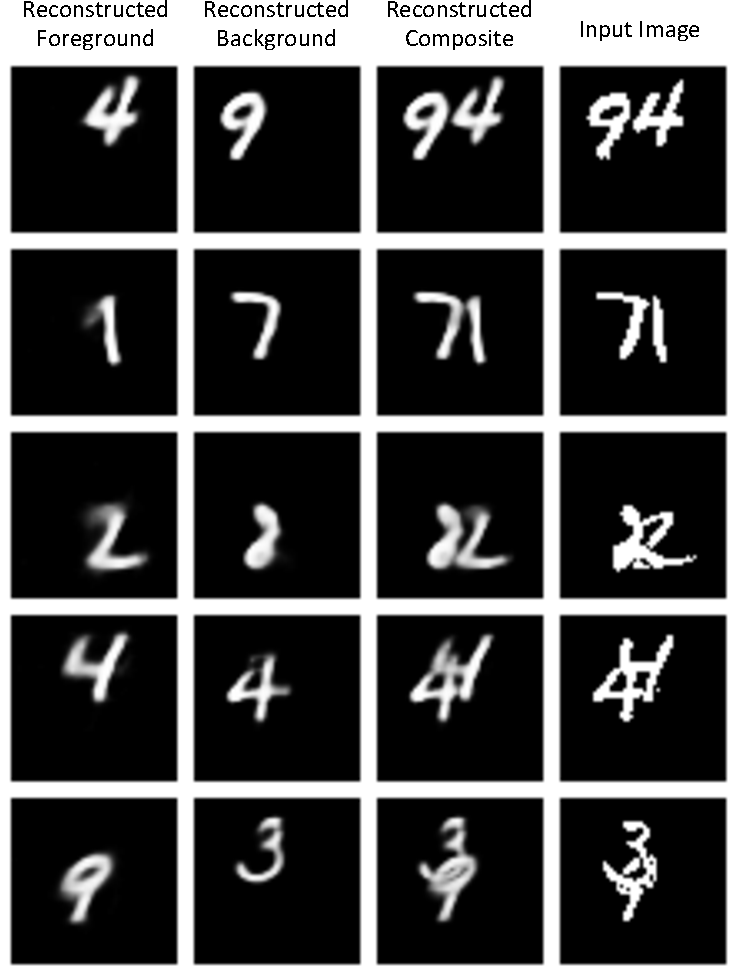
\includegraphics[width=0.3\linewidth]{figs/cstvae_reconstructions.pdf}
\label{fig:cstvae_reconstructions}
}
\end{center}
 \caption{hello}
\end{figure}




\subsection{Partially observed data}




\subsection{Supervised training}

compare accuracy on something



\subsection{With Textures???}












